We need the signaling proxy to translate the information exchange concerning the establishment and control of a communication session. The specific problems related to this component are repeated below:

\begin{itemize}
\item{How to authenticate users?}
\item{How to translate the signaling?}
\item{How to handle negotiating the \gls{sdp}?}
\end{itemize}

\section{Authentication}
VA supports authentication by username/password, which is trivial to do on the web. Therefore, authentication is not a problem. We can simply transmit the user's credentials using a secure connection over HTTPS.

\section{Signaling}
Implementing signaling for WebRTC using the H2O distributed computing framework used in VA, is beyond the scope of this thesis. Therefore, I've chosen to look at more common signaling scenarios. The most used signaling protocol for enterprise communication applications is the SIP protocol. In the report by 3GPP\cite{3gpp-wrtc-access-ims} on integrating WebRTC with IMS mentioned in the background chapter, they proposed to use SIP over WebSockets on the client side. This is a good solution, especially since WebSocket has very low average latencies\cite{websocket-overhead}. This means we only have to translate between SIP over WebSockets and the SIP protocol in our proxy. We can do this by using the SIP Proxy from the webrtc2sip gateway.

\section{SDP}
SIP is used to deliver the SDP, which we are required to exchange in WebRTC. \gls{sdp} is an old format used in the \gls{voip} world, therefore the re-use of \gls{sdp} is supposed to save time, but the anatomy of a \gls{sdp} is complex and under constant development because \gls{ietf} frequently updates the parameters to include. All the information has to be exactly right, or it will be rejected by the browser. It is highly unlikely that the current specification of \gls{sdp} will work with any older implementation found in any enterprise communication system. In order to establish a secure session, the following information has to be exchanged in addition to details about the media:

\begin{itemize}
\item{ICE username}
\item{ICE password}
\item{List of possible ICE candidates}
\item{DTLS fingerprint}s
\end{itemize}

We need to create methods for generating and manipulating the \gls{sdp} in this component.

\section{Experiments}
\label{sec:experiments}
By using the sipML5 client and the webrtc2sip gateway, I investigated whether it is possible that a WebRTC application using a SIP stack for JavaScript running over WebSockets interoperates with a desktop SIP client. By testing and evaluating this behavior, I will have confirmed that the proposed signaling component works.

Test setup:
\begin{itemize}
\item Chrome browser
\item sipML5 client (WebRTC) with RTCWeb Breaker enabled in expert mode
\item webrtc2sip gateway
\item SIP2SIP communication service\footnote{https://mdns.sipthor.net/register\_sip\_account.phtml}
\end{itemize}
I tested this locally with a range of different SIP clients:

\begin{table}[h]
\resizebox{\textwidth}{!}{%
\begin{tabular}{|p{1.3cm}|l|l|p{4cm}|p{4cm}|p{5cm}|}
\hline
SIP desktop clients & Audio & Video  & Perceived delay                                                                                         & Quality                                                  & Comments                                                                                                            \\ \hline
Ekiga               & g.711 & failed & none                                                                                            & good audio quality                                       & did not get video working                                                                                           \\ \hline
Zoiper              & g.711 & vp8    & none for audio, video took approximately 5 seconds to appear, but then it was a live connection & good audio quality, huge packet loss on the video stream & good audio quality, but poor video quality                                                            \\ \hline
Jitsi               & g.711 & failed & none                                                                                            & good audio quality                                       & connection failed every time the application tried to negotiate a video codec, but worked fine when disabling video \\ \hline
Blink               & opus  & failed & none                                                                                            & good audio quality                                       & did not get video working                                                                                           \\ \hline
\end{tabular}
}
\caption{WebRTC client interaction with SIP desktop clients using the webrtc2sip gateway.}
\label{tbl:sip-client-webrtc-interaction}
\end{table}

In Table \ref{tbl:sip-client-webrtc-interaction} the audio and video columns refer to the mutually agreed upon codec to be used during the signaling process. Since g.711 is the most preferred codec to be used in \gls{voip} systems, it is natural that audio most often defaults to this codec. In Figure \ref{fig:wireshark-sip-call-flow} we can see an analysis of the SIP call flow. We can see the call setup and the codecs which were offered. The codec used in this case was g.711 for audio. Acknowledgement of the hang up is sent last.

\begin{figure}[here]
\centerline{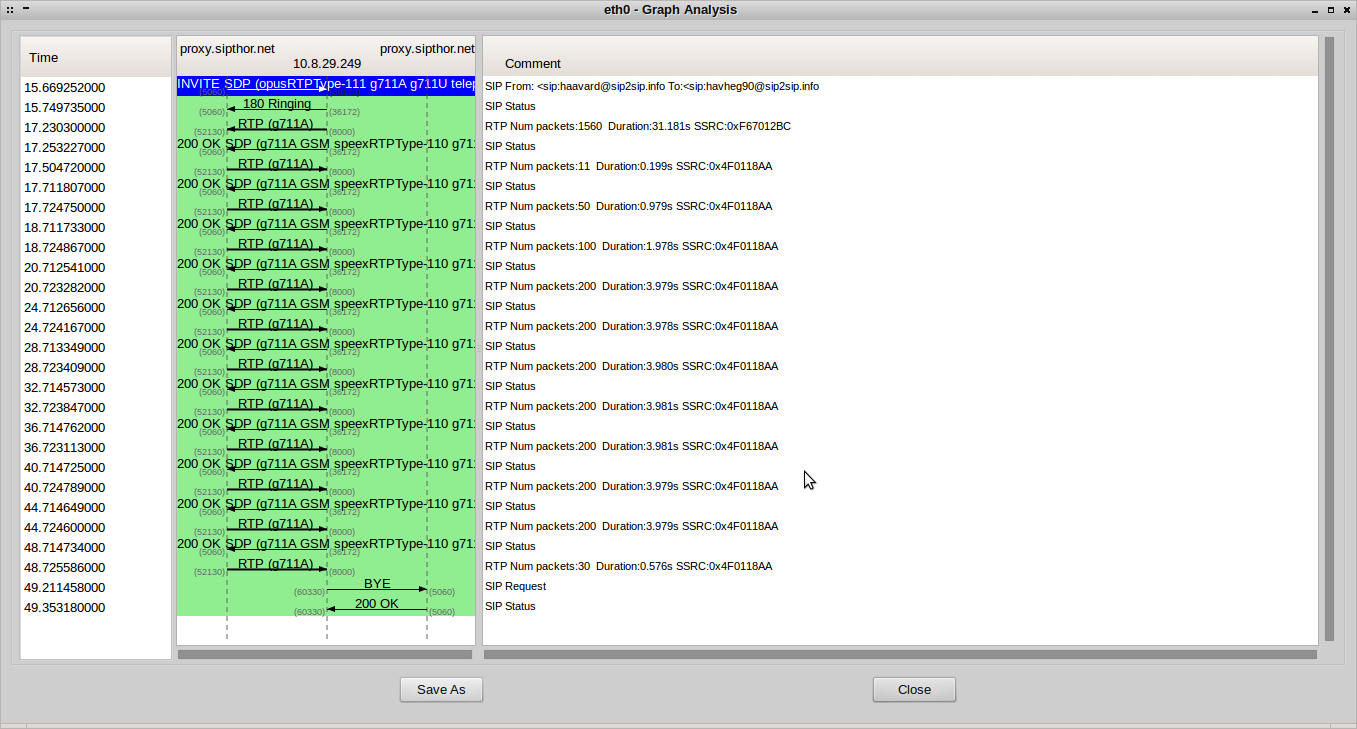
\includegraphics[width=\textwidth]{call-flow.png}}
\caption{Wireshark SIP call flow}
\label{fig:wireshark-sip-call-flow}
\end{figure}

\newpage
Experiments with audio went well, but video conferencing were not very successful. It was difficult to get a normal video session to work for various reasons, one of them being problems with the \gls{sdp}, which was mentioned earlier as a probable outcome. Below is an error message from a failed SDP exchange:

\begin{quote}
Failed to set remote offer sdp: Called with a SDP without crypto enabled. -from WebRTC Internals
\end{quote}

The one SIP client that did manage to get a working video session using the VP8 codec had a very high packet loss, as seen in Figure \ref{fig:wireshark-sip-call}. I did not find a good explanation for this, since the experiment was done on a really high-bandwidth connection. It seems from the experiments that the SIP proxy works, but it doesn't handle different implementations of SDP very well.

\begin{figure}[here]
\centerline{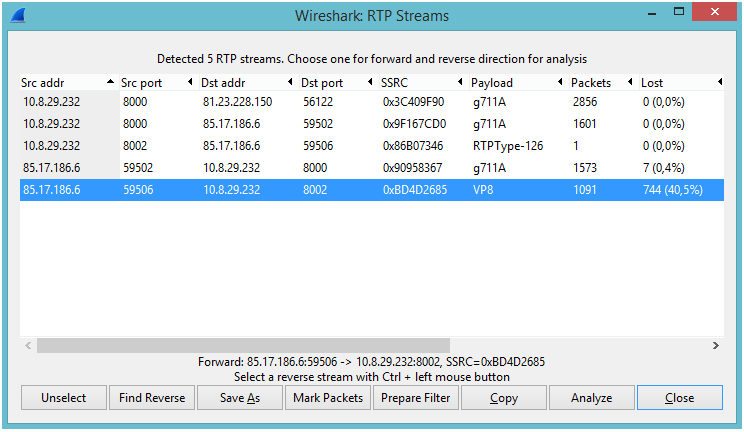
\includegraphics[scale=0.6]{wireshark-rtp.png}}
\caption{Wireshark analysis of a SIP call}
\label{fig:wireshark-sip-call}
\end{figure}

\newpage
\section{Summary}
For deriving general guidelines and for testing purposes, it's better to envision that our enterprise communication system uses the SIP protocol for signaling rather than VA's H2O. In this chapter we tested the sipML5 client, which is essentially a WebRTC client using SIP over WebSockets for signaling. The SIP proxy from webrtc2sip worked good for audio, but there were some problems negotiating video, possibly due to different implementations of the SDP. We can still use the SIP Proxy for signaling, but we should improve handling of the SDP. Another thing is that since SIP is mainly used to deliver the SDP, we should create an additional service to authenticate the users over a secure connection.